\usechapterimagetrue
\chapterimage{nasa.jpg} % Chapter heading image
\chapter{Channel coding}
\usechapterimagefalse

In the previous chapter we investigated the source coding problem. That is, given a source and some noiseless means of communication, the problem is to encode the source in such a way that we minimize the usage of the noiseless communications channel while we allow the receiver to recover the message. Here we will investigate a dual problem, the problem of transmitting a uniform source over a noisy channel. This problem, is the problem that your mobile phone faces each time that it wants to exchange information with the nearest base station, or the problem that your ADSL router faces to transmit information over fiber. It is also the same problem that your computer faces when it wants to store information on a disk in such a way that it can be recovered at a later time. This is as we see a very relevant problem. We won't have the time to dig into great depth, but the menu should allow you to get a solid understanding of the mathematical foundations and a glimpse about how we tackle it currently. In the figure above, you can see the XXXX space XXX. As you can imagine, the bandwidth of the communications channel linking it with earth is very limited, the information we want to exchange precious and the channel rather noisy. Space exploration has been one unexpected driver of progress for pushing the limits of error correcting codes. (why error correting?)
\booksection{The communications problem}
\label{sec:comprob}
\begin{figure}[h!]
\begin{center}
\def\svgwidth{\columnwidth} 
\input{figures/shannoncom.pdf_tex}
\end{center}
\caption[Communications system diagram.]{This figure reproduces the communications system diagram introduced by Shannon~\cite{Shannon_48}.}
\label{fig:shannoncom}
\end{figure}
Let us first of all, depict the building blocks of an idealized communications problem. Our description parallels the one of Shannon~\cite{Shannon_48}, see in Fig.~\ref{fig:shannoncom} a graphical representation. The figure shows five entities: an information source, a transmitter, a noise source, a receiver, and a destination. The communications scheme works as follows: 

First the information source generates a message $m$ from a set of possible messages $M$. Then, the transmitter takes $m$ and encodes it into $n$ channel symbols. We define the coding rate $R$ as:

\begin{equation}
R=\frac{\log M}{n}
\end{equation}

\begin{exercise}
Suppose that we want to transmit a message from a set of $16$ messages that a source will choose uniformly at random. We have two channels available, both are noiseless, one allows to transmit one bit per channel use and we can use it once per second. The second channel allows to transmit two bits per channel use and we can use it once per minute. Over which channel can we communicate at a higher rate? How does time influence this number?
\end{exercise}
The channel is a physical medium of transmission. Mathematically, we can model it as a system taking symbols from input alphabet $\mathcal{X}$ to symbols of output alphabet $\mathcal{Y}$ and characterized by a transition probability matrix that maps the probability of every symbol $y$ if symbol $x$ is sent. The receiver tries to undo the encoding given the noisy received signal and at the end of the scheme the destination receives the ${\hat{m}}$ possibly identical to $m$.

We define $C$, the capacity of a channel, as the maximum mutual information for all possible input distributions: 

\begin{eqnarray}
\label{eq:capform}
C = \max_{p(x)} I(X;Y)
\end{eqnarray}

\booksection{Refresher on linear algebra}

\booksection{Linear codes}
%\booksection{Detection, correction and minimum distance}
\booksection{Converse theorem for noisy channel coding}
The converse statement follows from Fano's inequality \cite{Fano_61}. The intuition behind this part is that if we think of an encoding that achieves a vanishing error probability, then necessarily $R<I(X;Y)$~\cite{Cover_91}. 

The past sections have been devoted to schemes that achieve a compression rate slightly larger than the entropy. We have called these schemes optimal. We also discussed that codes that have no error have an average length bounded from below by the entropy. In this section we will investigate what happens if we can tolerate some error. Surprisingly, we can not do much better than entropy. 

Let us first introduce Fano's inequality as it will be the main tool in our argument. Suppose that we want to guess the value of random variable $X$ and we have access to random variable $Y$, let us call $\hat X=g(Y)$ the random variable that characterizes the guess. We denote by $E$ the random variable that takes value 1 if $X=\hat X$ and 0 when $X\neq\hat X$. we can now state Fano's inequality:
\begin{theorem}[Fano's inequality]
Let $X,Y$ be two random variables and $\hat X=g(Y)$ for some function $g:\mathcal Y\mapsto\mathcal X$ and let $E=I(X=\hat X)$. Then:
\begin{equation}
H(X|Y)\leq H(E) + p_E(E=1)\log(|\mathcal X -1|)
\end{equation}
\end{theorem}
\begin{proof}
Let us first expand $H(X,E|Y)$ in two different ways applying the chain rule. First:
\begin{align}
H(E,X|Y) &= H(E|Y)+H(X|E,Y)\\
         &\leq H(E) + H(X|E,Y)\\
         &= H(E) + p_E(0) H(X|E=0, Y) + p_E(1)H(X|E=1,Y)\\
         &= H(E) + p_E(1)H(X|E=1,Y)\\
         &\leq H(E) + p_E(1)\log(|\mathcal X|-1)
\end{align}
where the first equality follows from the chain rule, the first inequality since conditioning reduces entropy, the second equality follows from application of the definition of conditional entropy and the second one since in the event that the error is zero, there is no uncertainty on the value of $X$, the last inequality follows since entropy can never be larger than the logarithm of the number of outcomes.

Let us note that $H(E,X|Y)$ can also be expanded as:
\begin{align}
H(E,X|Y)&=H(X|Y)+H(E|X,Y)\\
        &=H(X|Y)
\end{align}
where the first equality follows from the chain rule and the second because if both $X$ and $Y$ are known, then $E$ is also known.

The proof ends by joining \eqref{} with \eqref{}
\end{proof}
\begin{exercise}
In \eqref{}, we have that $H(X|E=1,Y)\leq \log(|\mathcal X|-1)$. Why can we remove one outcome from the alphabet of $X$?
\end{exercise}
\booksection{Hamming codes}

%\booksection{Random codes}
\booksection{Sketch of the noisy channel theorem}

The capacity of a channel specifies the maximum rate at which a source can be reliably sent through a channel. On the other hand, no source with a rate over the capacity of the channel can be sent with a vanishing error probability.

\begin{figure}
\begin{center}
\def\svgwidth{\columnwidth} 
\input{figures/channel.pdf_tex} 
\caption[Jointly typical sequences]{Graphical representation of the input and output typical sequences. A good encoding chooses as codewords a subset of the input typical sequences that produces disjoint sets of output typical sequences.}
\label{fig:channel}
\end{center}
\end{figure}

A sketch of the proof would be as follows. Encoder and decoder share a code-book of $2^{nR}$ codewords chosen within the $2^{nH(X)}$ typical sequences~\cite{Massey_77}. The encoder sends a codeword ${x}$ drawn with uniform probability. The decoder outputs a word $\hat{{x}}$ jointly typical with the received word ${y}$. It declares an error if ${x}$, ${y}$ are not jointly typical and a decoding error can occur if there exists ${x}'\neq {x}$ jointly typical with ${y}$. We know by Eq.~\ref{eq:jointtypical} that the probability of non-joint typicality for long enough $n$ can be made as small as desired. %We can bound the second source of error $p_e$ as well:

%\begin{eqnarray}
%p_e &\leq&  \left( 2^{nR}-1 \right) \frac{2^{n(H({XY})-\delta )}}{2^{n(H(X)-\delta )}2^{n(H(Y)-\delta )}}\nonumber\\
%     &\leq & 2^{-n(I(X;Y)-R-3\delta)}
%\end{eqnarray}
%\noindent in the first inequality we have bounded the error probability as the probability that one among the $2^{nR-1}$ remaining codewords belongs to the set of jointly typical sequences. The error probability vanishes only if $R<I(X;Y)$. However, we did not impose any condition on the $p(x)$ in the above discussion. In other words, if we choose the distribution that maximizes $I(X;Y)$, the typical sequence encoding achieves the capacity of the channel.

The intuition behind the achievability proof is simple. The decoder has access to two sets: the set of sequences jointly typical with ${y}$, and the set of codewords. If the intersection is to be a single word, every codeword has to be jointly typical with a disjoint set of typical output words. 

Approximately, every codeword is jointly typical with $2^{nH(Y|X)}$ words. Then the number of jointly typical output words with input codewords is upper bounded by $2^{nR+nH(Y|X)}$, where $R$ is the coding rate. This number should be much smaller than the total number of typical sequences $2^{nH(Y)}$:
 
\begin{equation*}
2^{nR+nH(Y|X)} < 2^{nH(Y)}
\end{equation*}

\noindent which operating returns the expected result:

\begin{equation*}
R < I(X;Y)
\end{equation*}

In conclusion, as long as the coding rate is below the mutual information between input and output for $n$ long enough we can construct a code that allows the decoder to distinguish between codewords with a vanishing probability of error.

\booksection{The capacity of some basic channels}

\subsection{Binary Symmetric Channel}
In the {BSC} the binary elements or bits are either perfectly transmitted with probability $1-p$ or flipped with probability $p$. 

Let us first find the mutual information between the input $X$ and the output $Y$~\cite{Cover_91}::

\begin{figure}[h]
\begin{center}
\def\svgwidth{\columnwidth} 
\input{figures/bsc.pdf_tex} 
\caption{Binary Symmetric Channel.}
\label{fig:bsc}
\end{center}
\end{figure}
%\begin{proof}

\begin{eqnarray}
I(X;Y) &=& H(Y) - H(Y|X) \\
         &=& H(Y) - \sum_x p(x)H(Y|x) \\
         &=& H(Y) - \sum_x p(x)H(p,1-p) \\
         &=& H(Y) - H(p,1-p)\sum_x p(x) \\
         &\leq & 1 - H(p,1-p)\label{eq:bscC} 
\end{eqnarray}

We obtain the capacity by finding the maximum of the mutual information for all possible input distributions. It can be easily verified that the the uniform distribution reaches the upper bound in Eq.~\ref{eq:bscC} and the capacity of the {BSC} is one minus the binary entropy of $p$.
%and this capacity is achieved for $p(X=0)=p(X=1)=\frac{1}{2}$.
%\end{proof}

\subsection{Binary Erasure Channel}
The {BEC} was introduced by Elias in his famous paper "Coding for Two Noisy Channels"~\cite{Elias_55}. The {BEC} has two input elements while the output alphabet is composed of three elements: 0, 1, and $e$, which stands for an erasure in the channel. In this channel the bits are either correctly transmitted with probability $1-p$, or are erased with probability $p$. 

We can first find $H(X|Y) $: 

\begin{figure}[h]
\begin{center}
\def\svgwidth{\columnwidth} 
\input{figures/bec.pdf_tex} 
\caption{Binary Erasure Channel.}
\label{fig:bec}
\end{center}
\end{figure}

%\begin{proof}

%\begin{eqnarray}
%\label{eq:beccap1}
%H(Y) &=& H((1-p )(1-\pi ),p , (1-p ) \pi) \\
%        &=&  H(1-p , p ) + (1-p ) H(\pi, 1 - \pi )
%\end{eqnarray}
%\begin{eqnarray}
%\label{eq:beccap2}
%H(Y|X) &=& (1 -\pi )H(p, 1-p ) + \pi H(p, 1- p) \\
%           &=& H(p, 1- p)
%\end{eqnarray}
\begin{eqnarray}
\label{eq:beccap}
H(X|Y) &=& \pi (1-p )H(X|Y=0) \nonumber\\
           && + \left( \pi\, p +(1-\pi)p\right) H(X|Y=e)\nonumber\\
           && + (1-\pi)(1-p)H(X|Y=1) \\
           &=& p
\end{eqnarray}
\noindent where $p(X=0)=\pi$.The second equality holds from $H(X|Y=1)=H(X|Y=0)=0$ and $H(X|Y=e)=1$. We can now plug Eq.~\ref{eq:beccap} in Eq.~\ref{eq:mutualinformation} and bound from above the mutual information:
\begin{eqnarray}
I(X;Y) &=& H(X) - H(X|Y) \\
         &=& H(\pi, 1-\pi) - p\\
         & \leq & 1 - p\label{eq:becineq}
\end{eqnarray}
\noindent equality in Eq.~\ref{eq:becineq} is achieved again by the uniform distribution. That is, for $\pi=\frac{1}{2}$.
%\end{proof}

%\begin{eqnarray}
%C = \max_{p(x)} I(X;Y) = 
%\end{eqnarray}

It might seem that the capacity of a {BSC} that flips bits with probability $p$ is greater than the capacity of a {BEC} that erases bits with probability $p$. Fig.~\ref{fig:becbsc} shows that it is the opposite situation. On the range $p\in\left( 0,0.5\right)$, the capacity of the {BEC} is greater than the capacity of the {BSC}. Bits on the {BEC} are either perfectly known or perfectly unknown, however, it is not possible to distinguished flipped bits from correct bits in the {BSC}.

\begin{figure}[h]
\begin{center}
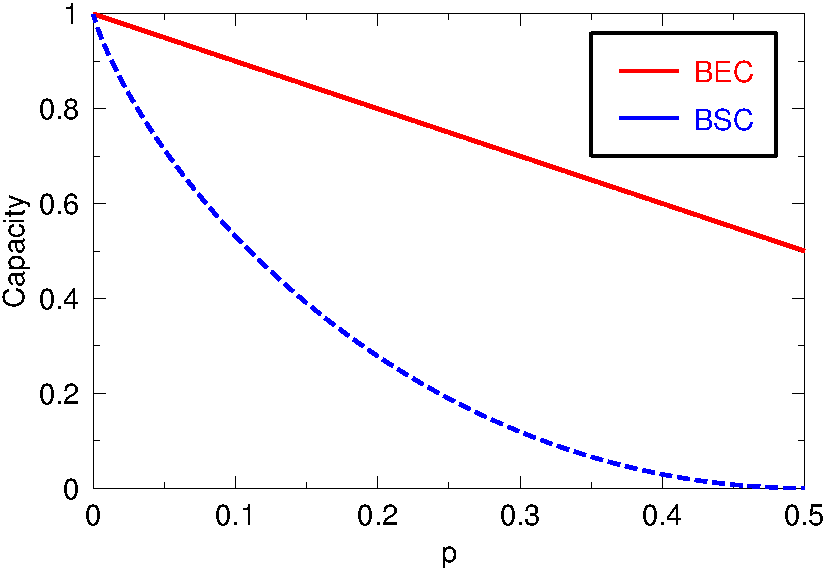
\includegraphics[width=\linewidth]{figures/becbsc.pdf}
\caption{The capacity of the BEC and BSC.}
\label{fig:becbsc}
\end{center}
\end{figure}

\booksection{Exercises}
\booksection{Further reading}
Chapter 7 in \cite{Cover_91}. 
